\section{Test}

\subsection{Codice}
Lato codice è stata testata la RestApi.
Di eseguito alcuni screenshot di esempio.

\begin{figure}[H]
	\centering
	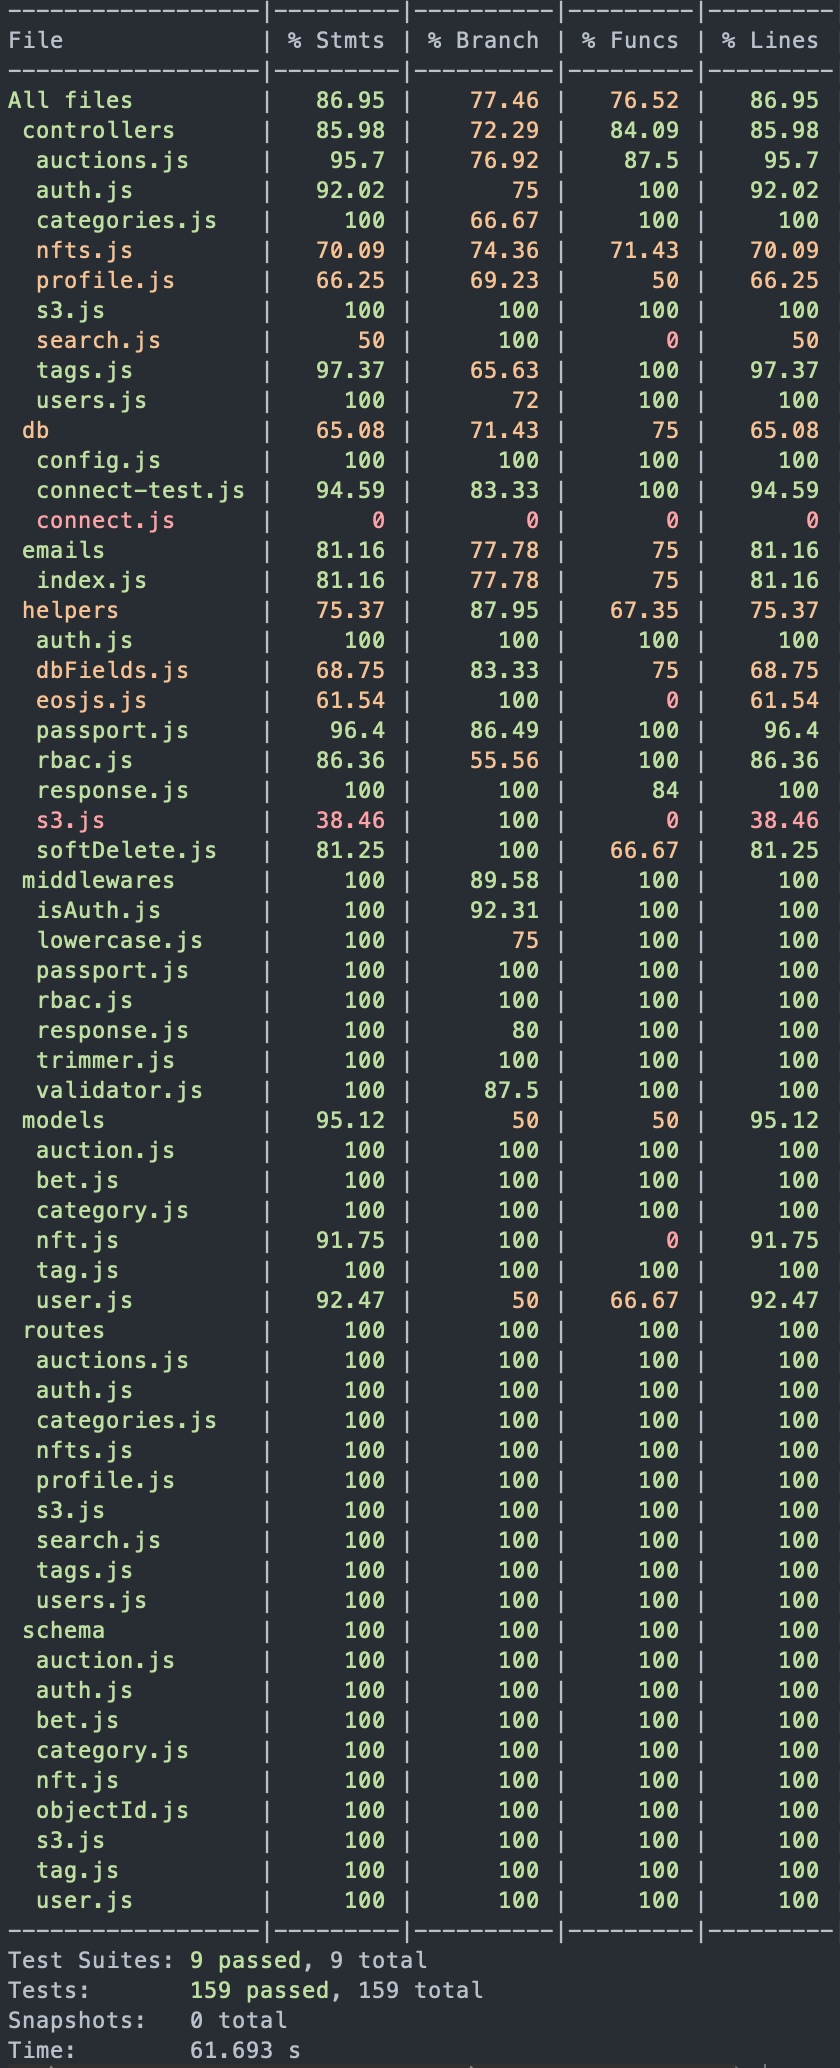
\includegraphics[width=0.40\textwidth,keepaspectratio]{api-test.jpg}
	\caption{Test coverage della RestApi}
	\label{fig:apiTest}
\end{figure}

\begin{figure}[H]
	\centering
	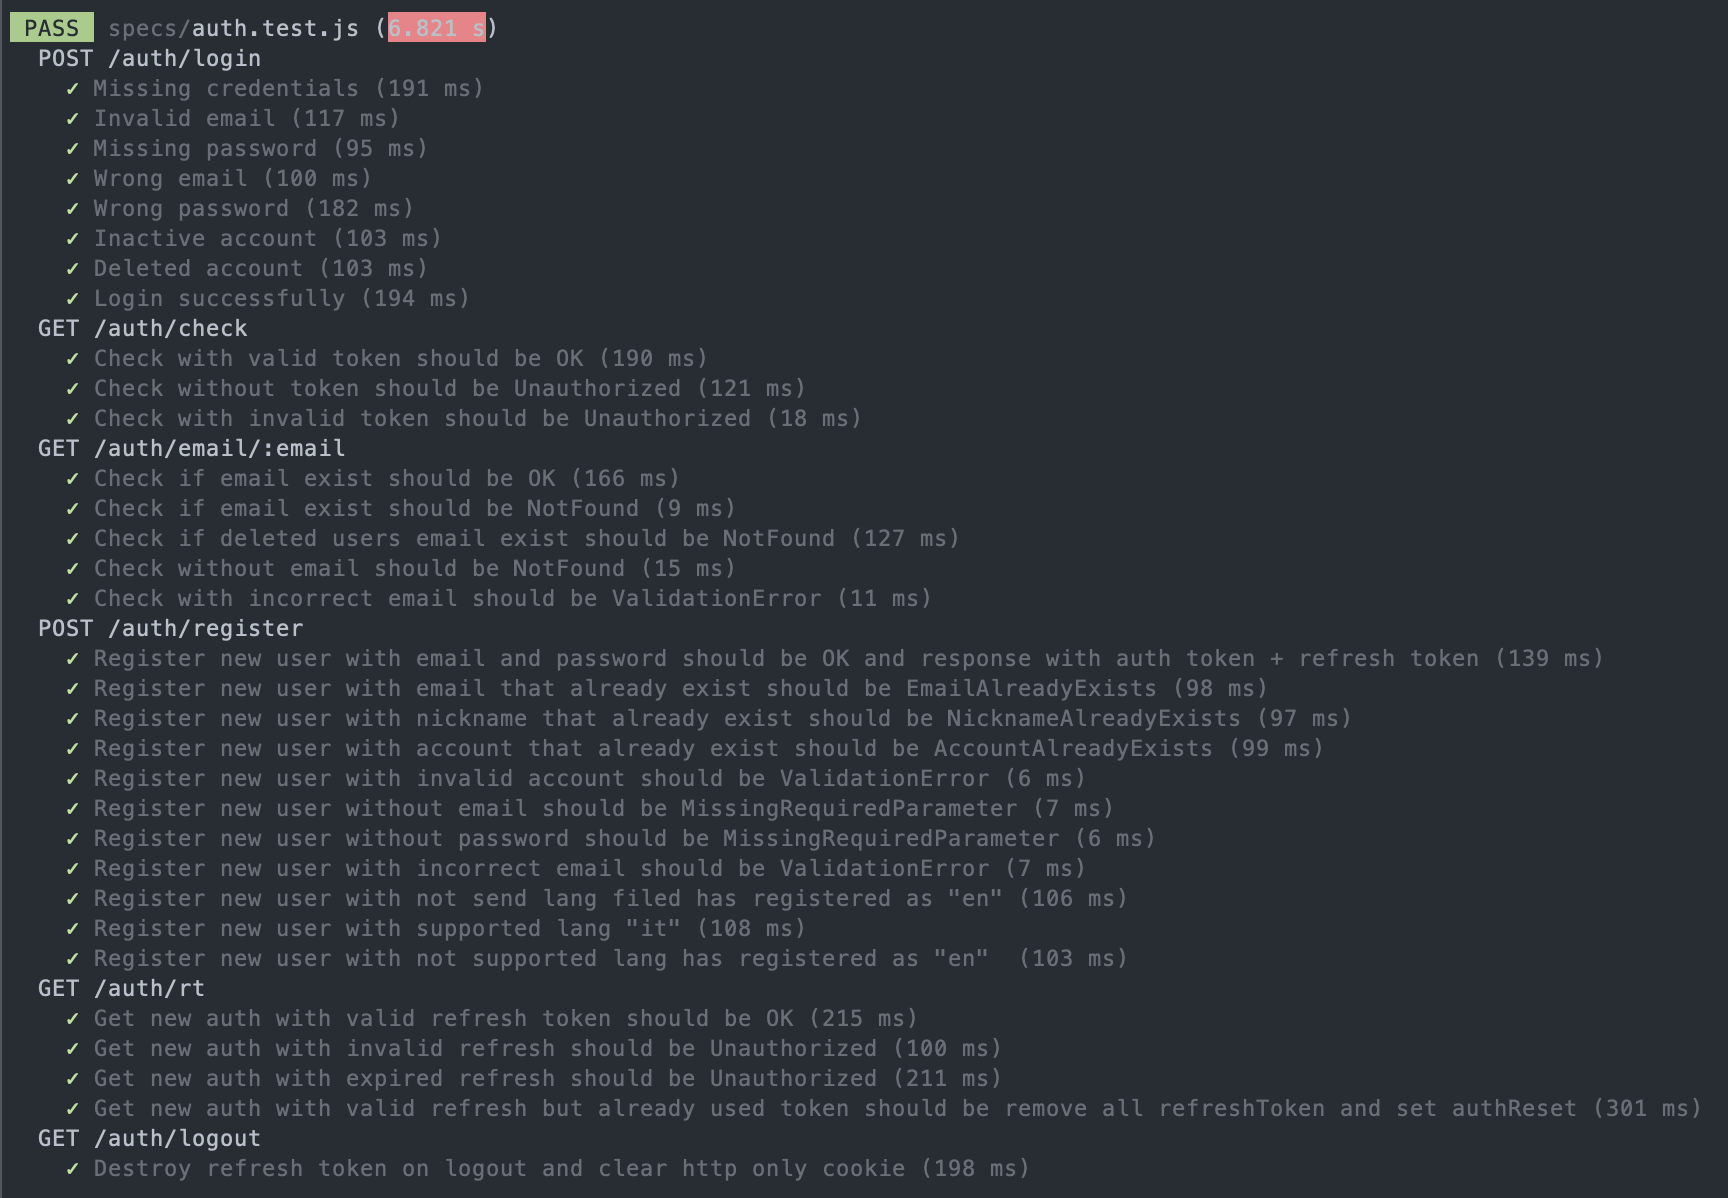
\includegraphics[width=\textwidth,keepaspectratio]{auth-test.jpg}
	\caption{Test dell'endpoint /auth per l'autenticazione}
	\label{fig:authTest}
\end{figure}

\begin{figure}[H]
	\centering
	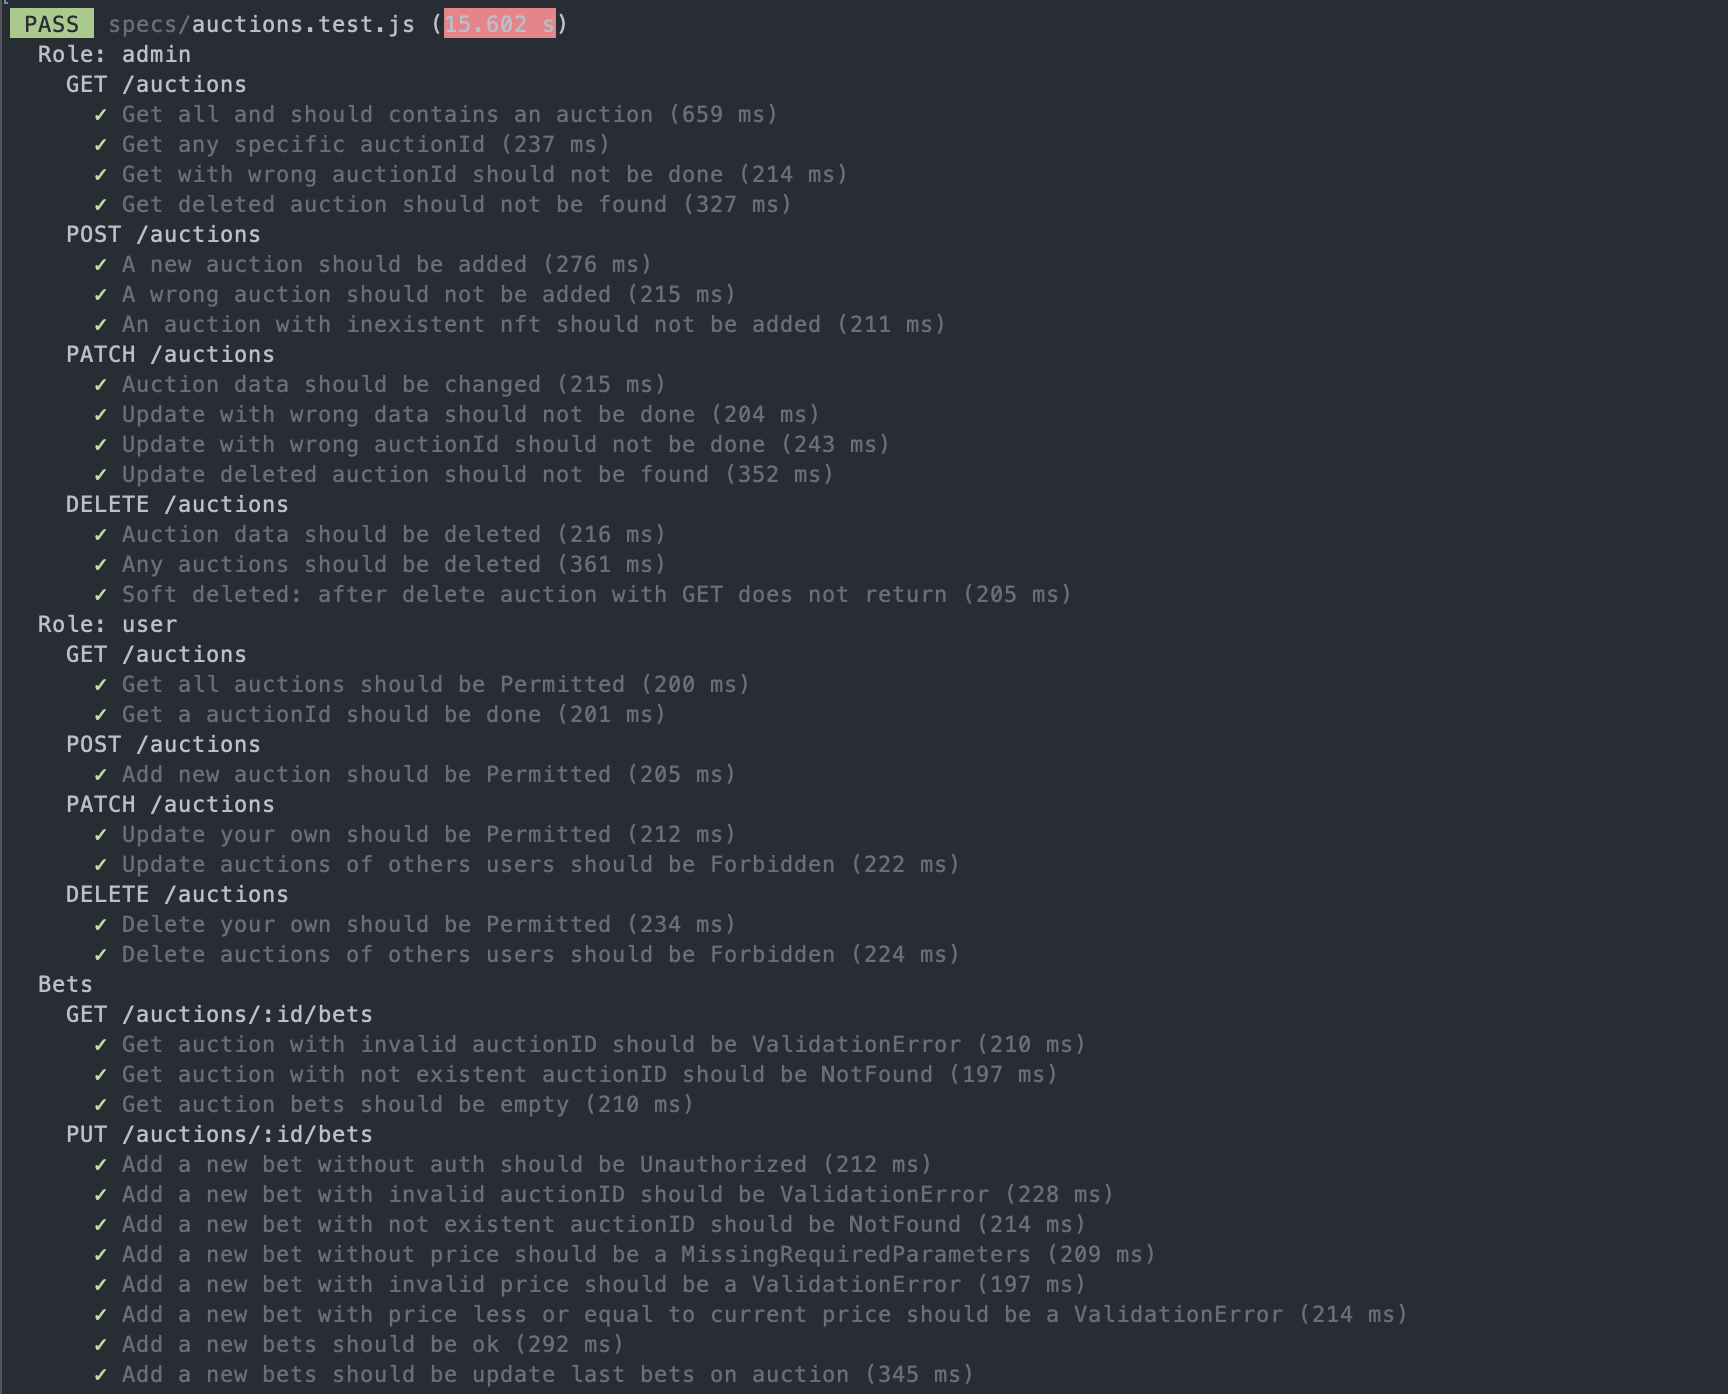
\includegraphics[width=\textwidth,keepaspectratio]{auctions-test.jpg}
	\caption{Test dell'endpoint /auctions delle aste}
	\label{fig:auctionsTest}
\end{figure}

\clearpage

\subsection{User Experience}
Fatto provare il prototipo
sono emerse correzioni